\chapter{PLANTEAMIENTO DEL PROBLEMA}
\section{Descripción de la Realidad Problemática}

En la actualidad, el emprendimiento es el impulso de muchas personas para salir adelante. Desde crear innovar en productos y servicios, hasta crear nuevas maneras de ejercer actividades cotidianas, gracias a ideas nacidas a partir de querer cubrir una necesidad.

De acuerdo al reporte de Global Entrepreneurship Monitor (GEM) del 2014, el 50.6\% de la población del Perú entre 18 y 64 años tenía la expectativa de iniciar un emprendimiento dentro de los siguientes tres años, del cual el 62.3\% de la población de dicho rango de edad tiende a ser más optimista en su percepción de oportunidades. Asimismo, según informa la Cámara de Comercio de Lima, la iniciativa emprendedora responde más a la identificación de una oportunidad de negocio que a una falta de oportunidad de empleo \parencite{cr_gestion2015emprendper}. Sin embargo, en un estudio más reciente basado en una encuesta realizada a residentes peruanos entre junio y julio del 2017 desarrollada por el equipo GEM Perú y ESAN a 2080 personas entre el mismo rango de edad, el 24.6\% de emprendimientos se encontraba en fase temprana, es decir, representaba una dificultad para el emprendedor peruano llegar a etapas más avanzadas como un emprendimiento establecido (negocios con más de 3.5 años, que representan solo el 7.4\% para Perú), ubicando así al país en la posición 25 de 54 economías a nivel mundial \parencite{cr_gestion2018emprend}. En la Figura \ref{1:fig} se aprecian algunas ratios del estudio. %\medskip

\begin{figure}[h]
	\begin{center}
		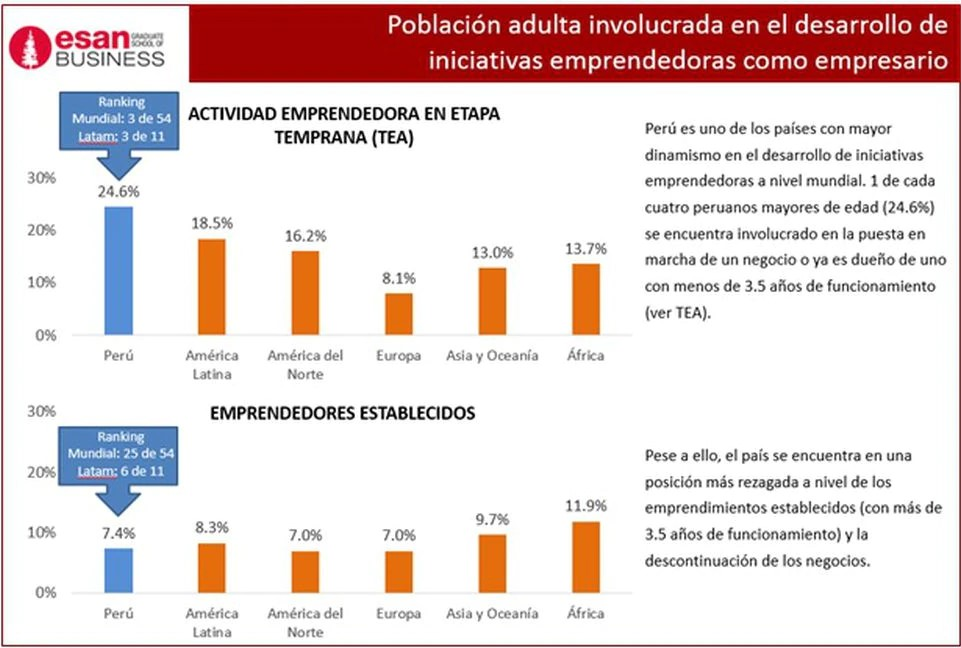
\includegraphics[width=0.65\textwidth]{1/figures/cuadro_esan.jpg}
		\caption[Resultados y ratios obtenidos en la encuesta por GEM y ESAN]{Resultados y ratios obtenidos en la encuesta por GEM y ESAN.\\
		Fuente: \cite{cr_gestion2018emprend}. \textit{Perú es el tercer país con mayor cantidad de emprendimientos en fase temprana a nivel mundial}.}
		\label{1:fig}
	\end{center}
\end{figure}

Los resultados desfavorables tienen como base el ecosistema poco beneficioso para los emprendimientos que permitan establecerse en su entorno nacional, con condiciones asociadas al acceso de financiamiento, políticas gubernamentales que alienten la implementación de Innovación y Desarrollo en las empresas, acceso a infraestructura física y asesoría a nivel comercial y profesional, como sostiene el investigador del equipo GEM Perú Carlos Guerrero \parencite{cr_gestion2018emprend}. La Asociación de Emprendedores de Perú (ASEP) afirma, asimismo, que en la región solo se invierte el 1.5\% del PIB en actividades de ciencia, tecnología e innovación, y las limitaciones son dadas por barreras burocráticas ejercidas por el Gobierno y el sector privado \parencite{cr_aep2018emprend}. En adición a esto, otras razones que representan barreras para emprender son la falta de conocimientos en la iniciación de un negocio, su tramitación, la fuente de financiamiento del proyecto o búsqueda de inversionistas, la cultura, la falta de fomento de emprendimiento y la falta de red de contactos \parencite{cr_sandoval_barreras}.

Ante estas limitaciones, en la actualidad muchos emprendedores se ven forzados a mostrar sus proyectos al público en la Internet con el fin de captar personas interesadas en ayudarlos en el financiamiento de estos. Por ello, se han creado plataformas web con el fin de permitir la interacción entre los proyectos publicados en un determinado tiempo, el cual puede variar entre 30 y 120 días, y la comunidad en general que desee colaborar con una cantidad de dinero para su financiamiento. El sitio web solo servirá para mostrar los proyectos presentados a detalle por los creadores y la promoción de estos al público. La idea es que, al término de este plazo de tiempo, el proyecto sea financiado y se logre convertir en una realidad. A esta práctica se le conoce como crowdfunding \parencite{cr_uc_crowdfunding}.

En Latinoamérica, son muy pocos los países los que se incorporan en el crowdfunding, entre los principales se destacan Chile, México, Argentina y Brasil. Sin embargo, el modelo funciona distinto a países de Norteamérica y Europa debido a la diferencia cultural y resistencia a su implementación por la poca confianza en el éxito de los proyectos. Por ejemplo, se encontró en dichos países que los proyectos audiovisuales, a pesar de encontrarse en desventaja que en sus pares europeos y norteamericanos, se estrenaron 4,135 títulos extranjeros en la región iberoamericana frente a 791 propios, de los cuales 162 fueron obras brasileñas y 131, argentinas, en el año 2015. Algunos de los factores principales fueron el apoyo de sus gobiernos, la masificación de las comunicaciones digitales y por ende, la participación activa de usuarios en redes sociales y el papel protagónico que toma el crowdfunding para apoyar estos proyectos (22,179 proyectos financiados con éxito en Kickstarter con más de 1 millón de dólares de recaudación en el 2017) \parencite{cr_lopezgolan2017crowdfunding}. Asimismo, en los últimos años se decidió seguir una manera muy similar a los modelos de Estados Unidos, basados en la creación de campañas de un emprendedor para obtener fondos para sus ideas con la moneda norteamericana pero limitados a las leyes económicas de cada país \parencite{cr_sl_crowdfundlatam}. En el caso del Perú, el crowdfunding existe y es apoyada por universidades y organizaciones sin fines de lucro, cuyo objetivo es generar empresas comerciales que aumenten la calidad de vida en la comunidad, además de convertir a las personas en socios financieros \parencite{cr_fernandezbedoya2020colecoperu}. Esta actividad es parte de uno de los 4 grupos básicos de economía colaborativa: el financiamiento colaborativo \parencite{cr_stokes2014coleco}.

Kickstarter e Indiegogo figuran entre los sitios web más conocidos de crowdfunding. El primero, desde su inicio en 2009, es una plataforma de financiamiento de proyectos creativos de todo tipo, los cuales incluyen películas, juegos, música, arte, diseño y tecnología. Actualmente, se han registrado más de 162 mil proyectos realizados, 16 millones de contribuyentes y 4,3 miles de millones de dólares fondeados \parencite{cr_kickstarter_about}. Utiliza un modelo de financiamiento llamado “todo o nada”, el cual consiste en que si un proyecto no alcanza su meta de financiamiento en un determinado plazo de tiempo, no se realiza ninguna transacción de fondos \parencite{cr_kickstarter_founding}. Si bien los patrocinadores apoyan estos proyectos por motivos personales y distintos para hacerlos realidad, ellos no obtienen la propiedad o los ingresos de los proyectos que financian, sino que los creadores conservan la totalidad de su trabajo \parencite{cr_kickstarter_press}.

De todas las categorías, los proyectos tecnológicos alcanzaron el ratio más bajo (20\%) al 2019, como se aprecia en la Figura \ref{1:fig2}.
\begin{figure}[h]
	\begin{center}
		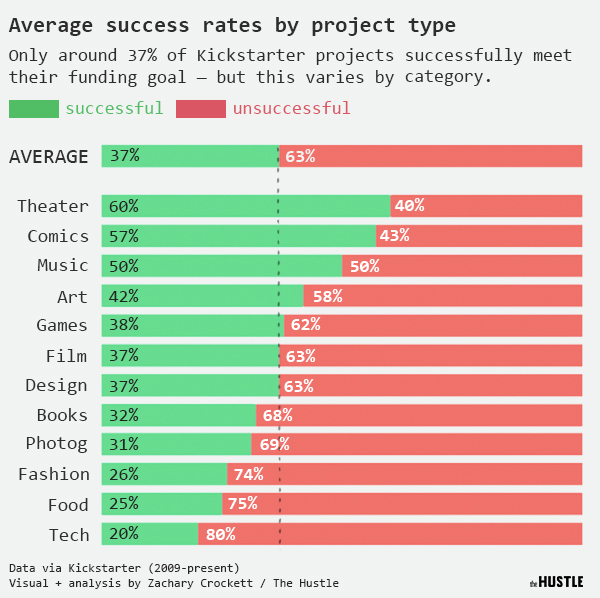
\includegraphics[width=0.55\textwidth]{1/figures/kickstarter_success_rate_2009_2019.jpg}
		\caption[Ratio de éxito de proyectos en Kickstarter desde 2009 hasta 2019 (Febrero)]{Ratio de éxito de proyectos en Kickstarter desde 2009 hasta 2019 (Febrero).\\
		Fuente: \cite{cr_hustle2019successrate}. \textit{What are your chances of successfully raising money on Kickstarter?}}
		\label{1:fig2}
	\end{center}
\end{figure}

Además de este problema, en general muchas veces las campañas fracasan por los valores incorrectos que toman sus variables, desde el contenido de la publicación hasta la comunicación de parte de los creadores con los patrocinadores. Es decir, el factor incertidumbre se vincula con la campaña cuando esta no resulta lo suficientemente atractiva por la ausencia de características que sí presentan los proyectos que fueron financiados.

Existen estudios previos para predecir la probabilidad de éxito de financiamiento para este tipo de proyectos utilizando técnicas de Aprendizaje Automático y Profundo. Sin embargo, la mayoría de los modelos predictivos entrenan usando solo una modalidad o utilizando la data de todas las categorías, originando una generalización en base al ratio global de éxito. Para la actual investigación, se implementó un modelo bajo un enfoque distinto y considerando solamente a proyectos de tecnología.

\section{Formulación del Problema}
Para la formulación de los problemas de la presente investigación, se elaboró un «árbol de problemas» (véase Anexo \ref{anexo1}).

\subsection{Problema General}
PG: \newcommand{\ProblemaGeneral}{
¿Es posible predecir el estado de financiamiento de proyectos de tecnología en sitio web de crowdfunding Kickstarter mediante un modelo de Aprendizaje Profundo Multimodal?
}
\ProblemaGeneral
\subsection{Problemas Específicos}
\newcommand{\Pbone}{
¿Qué alternativas se proponen en los trabajos previos para seleccionar características y desarrollar el marco de trabajo de la investigación?
}
\newcommand{\Pbtwo}{
¿Qué condiciones técnicas factibles de las propuestas de la literatura existen en el ambiente de desarrollo para implementar las características del modelo de Aprendizaje Profundo Multimodal?
}
\newcommand{\Pbthree}{
¿Cuál es el impacto que generarán las características consideradas en el desarrollo del modelo de Aprendizaje Profundo Multimodal?
}
\newcommand{\Pbfour}{
¿Qué alternativas analíticas existen para ayudar a los emprendedores y creadores de proyectos de tecnología en la toma de decisiones y estrategias de sus campañas?
}

\begin{itemize}
	\item PE1: {\Pbone}
	\item PE2: {\Pbtwo}
	\item PE3: {\Pbthree}
	\item PE4: {\Pbfour}
\end{itemize}

\section{Objetivos de la Investigación}
Para la formulación de los objetivos de la presente investigación, se elaboró un «árbol de objetivos» (véase Anexo \ref{anexo2}) 
\subsection{Objetivo General}
OG: \newcommand{\ObjetivoGeneral}{
Predecir el estado de financiamiento de proyectos de tecnología en sitio web de crowdfunding Kickstarter mediante modelo de Aprendizaje Profundo Multimodal.
}
\ObjetivoGeneral
\subsection{Objetivos Específicos}
\newcommand{\Objone}{
Analizar las alternativas propuestas en los trabajos previos para seleccionar características y desarrollar el marco de trabajo de la investigación.
}
\newcommand{\Objtwo}{
Evaluar la factibilidad técnica del ambiente de desarrollo para las características del modelo de Aprendizaje Profundo Multimodal bajo las condiciones de las propuestas de la literatura.
}
\newcommand{\Objthree}{
Examinar el impacto de las características consideradas en el desarrollo del modelo de Aprendizaje Profundo Multimodal.
}
\newcommand{\Objfour}{
Implementar herramienta analítica en tiempo real para ayudar a los emprendedores y creadores de proyectos de tecnología en la toma de decisiones y estrategias de sus campañas.
}

\begin{itemize}
	\item OE1: {\Objone}
	\item OE2: {\Objtwo}
	\item OE3: {\Objthree}
	\item OE4: {\Objfour}
\end{itemize}

\section{Hipótesis}

\subsection{Hipótesis General}
HG: \newcommand{\HipotesisGeneral}{
	El modelo de Aprendizaje Profundo Multimodal predecirá el estado de financiamiento de proyectos de tecnología en sitio web de crowdfunding Kickstarter.
}
\HipotesisGeneral
\subsection{Hipótesis Específicas}
\newcommand{\Hone}{
El análisis de las alternativas propuestas en los trabajos previos influirá en la selección de características y desarrollo del marco de trabajo de la investigación.
}
\newcommand{\Htwo}{
La factibilidad técnica del ambiente de desarrollo para las características del modelo de Aprendizaje Profundo Multimodal determinará la aplicabilidad de las condiciones de las propuestas de la literatura.
}
\newcommand{\Hthree}{
El modelo de Aprendizaje Profundo Multimodal se verá afectado por las características consideradas en su desarrollo.
}
\newcommand{\Hfour}{
La herramienta analítica implementada ayudará en tiempo real a los emprendedores y creadores de proyectos de tecnología en la toma de decisiones y estrategias de sus campañas.
}

\begin{itemize}
	\item HE1: \Hone
	\item HE2: \Htwo
	\item HE3: \Hthree
	\item HE4: \Hfour
\end{itemize}

Los problemas, objetivos e hipótesis descritas anteriormente se encuentran alineadas en la Matriz de Consistencia del Anexo \ref{anexo3}.

\section{Justificación de la Investigación}

\subsection{Teórica}
Esta investigación se realizó con la finalidad de aportar al conocimiento existente del problema de la predicción del estado de financiamiento de un proyecto en plataformas de crowdfunding como Kickstarter, pero considerando solo proyectos de la categoría Tecnología, cuyo ratio de éxito de 20\% la clasifica como la más baja de todas, criterio que también se menciona en la literatura por \cite{pr_lee2018contentDL}.

Para ello, el nuevo aporte aplicado a la investigación fue la implementación de un modelo de Aprendizaje Profundo Multimodal utilizando la información de la sección principal de la campaña (metainformación y descripción) y los comentarios de los patrocinadores como resultado de la interacción entre ellos y los creadores. Esta nueva perspectiva considera las 3 modalidades más utilizadas en los antecedentes bajo un modelo que solo fue desarrollado en 1 antecedente por \cite{pr_cheng2019deeplearning}, el cual utilizó solo modalidades de la sección principal (metainformación, descripción e imagen del proyecto).

\subsection{Práctica}
Muchos trabajos previos analizados en la literatura plantearon distintas soluciones para resolver el mismo problema. Sin embargo, a pesar de que sus resultados en su mayoría alcanzaron niveles de predicción por encima a los esperados por los autores, menos de la mitad (8 de los 18 antecedentes mencionados) llegaron a ejecutar la fase de Despliegue, es decir, no fueron puestos en producción para ser utilizados por otros usuarios, o se mencionaron que se convertiría en una tarea para trabajos a futuro.

Al culminar esta invesigación, se podrá utilizar el prototipo de un sistema que integra el modelo propuesto, el cual funciona en tiempo real capturando la información de las variables solamente recibiendo como entrada la URL del proyecto, con la finalidad de poder ser una herramienta analítica de ayuda en la toma de decisiones a emprendedores que buscan financiar sus proyectos de tecnología en Kickstarter. La retroalimentación será recíproca entre el usuario y el prototipo, ya que en la primera iteración, el creador tendrá una idea inicial del resultado de éxito de financiamiento que tendrá su campaña de acuerdo a la información actual presente en sus variables, y ante una respuesta adversa, podrá realizar las modificaciones respectivas en las modalidades entrenadas que tiene acceso (metainformación y descripción) para ejecutar nuevamente el prototipo, que ahora hará la predicción a partir de nuevos datos, de forma indefinida. De esta manera, se logrará crear una campaña más atractiva para los patrocinadores.

\subsection{Metodológica}
La implementación del modelo propuesto ayudará a los emprendedores y creadores a evaluar las campañas de sus proyectos a partir de la información vigente que sea capturada en tiempo real por el prototipo para predecir el estado de financiamiento.

Para ello, se utilizaron técnicas de Aprendizaje Profundo y Procesamiento de Lenguaje Natural entrenados con un conjunto de datos compuesto por 3 modalidades de proyectos en Kickstarter que fueron generados luego de un proceso de recolección de datos.

\section{Delimitación del Estudio}

\subsection{Espacial}
Para la presente investigación, se consideraron proyectos de tecnología de distintas ciudades y países, mayoritariamente del territorio de los Estados Unidos. Sin embargo, la información textual (descripción y comentarios) para la fase de entrenamiento solo se tómo en cuenta palabras en inglés.

\subsection{Temporal}
El periodo de tiempo abarcará desde el año 2009, fecha en el cual se tiene registrado los primeros conjuntos de datos de proyectos en Kickstarter hasta el mes de agosto del año 2019, últimos registros descargados hasta el inicio del presente trabajo.

\subsection{Conceptual}
Esta investigación se orientará en la implementación de un modelo que logre predecir si un proyecto de tecnología en el sitio web de crowdfunding Kickstarter será financiado o no. Para ello, se valió del uso de herramientas de Aprendizaje Profundo y Procesamiento de Lenguaje Natural para desarrollar los modelos de acuerdo a sus modalidades respectivas, así como el Aprendizaje Profundo Multimodal para consolidar estos conceptos.